\documentclass[11pt, a4paper]{article}
\usepackage[utf8]{inputenc}
\usepackage{amsmath}
\usepackage{amsfonts}
\usepackage[english]{babel}
\usepackage{float}
\usepackage[letterpaper,top=2.2cm,bottom=2.2cm,left=3cm,right=3cm,marginparwidth=1.75cm]{geometry}
\usepackage{graphicx}
\usepackage[colorlinks=true, allcolors=blue]{hyperref}
\usepackage{parskip}
\usepackage[style=ieee, backend=biber, language=english]{biblatex}
\addbibresource{Ref.bib}
\usepackage{authblk}

\title{\Large \textbf{Comparative analysis of \textit{Bacillus subtilis} genome-scale metabolic models (GEMs) using Flux Balance Analysis (FBA)}}

\author[1]{Gabriel Felipe Granados Ramírez}
\author[2]{Juan David Tibocha Bonilla}
\author[3]{César Augusto Vargas García}
\author[4]{Óscar Fernando Sánchez Medina}

\affil[1]{Pontificia Universidad Javeriana, Faculty of Science, Bogotá, Colombia}
\affil[2]{Lawrence Berkeley National Laboratory, Berkeley, California}
\affil[3]{AGROSAVIA, Corporación Colombiana de Investigación Agropecuaria, Mosquera, Colombia}
\affil[4]{Pontificia Universidad Javeriana, Faculty of Engineering, Bogotá, Colombia}

\date{}  

\begin{document}

\maketitle

\section{Abstract}

\textit{Bacillus subtilis} is a model organism and industrial production host for which fourteen genome-scale metabolic models (GEMs) have been reconstructed, developed independently and differing in size, nomenclature and annotation, leaving unclear which to prefer for a given task. We compared ten of them under a common M9 minimal medium, standardized to BiGG nomenclature and annotated with Systems Biology Ontology terms, across structural quality, growth on several carbon sources and in chemostat culture, central carbon fluxes, gene essentiality and Biolog substrate utilization. No reconstruction ranked first on every test, and structural quality proved largely independent of predictive accuracy: iYO844 scored highest on both quality and annotation yet performed mid-table functionally. The models also failed in shared ways, six of them overestimating growth through unrestricted use of the cytochrome caa$_3$ oxidase and six carrying no flux through the oxidative pentose phosphate pathway. Model selection should therefore follow the intended prediction task rather than a single quality score.

\section{Introduction}
\textit{Bacillus subtilis} is a widely studied Gram-positive bacterium, renowned for its metabolic versatility \parencite{su-2020}, its ability to grow on a wide range of substrates \parencite{mageshwaran-2014}, and its long-standing role as a model organism for the study of cell physiology, sporulation \parencite{tibocha-bonilla-2025}, and gene regulation \parencite{goelzer-2008}. It is also extensively used in industrial biotechnology for the production of vitamins, enzymes, and recombinant proteins due to its efficient secretion system \parencite{liu-2025} and generally recognized as safe (GRAS) status \parencite{akinsemolu-2024}. With the advent of modern sequencing technologies, the genome of \textit{B. subtilis} was first fully sequenced and annotated in 1997, revealing a circular chromosome of approximately 4.2 Mb encoding around 4,200 protein-coding genes \parencite{kunst-1997}. Since then, its genome has undergone multiple rounds of reannotation and refinement, becoming one of the most comprehensively characterized bacterial genomes \parencite{errington-2020}. Consequently, \textit{B. subtilis} has been a major target of metabolic engineering efforts aimed at optimizing bioproduction processes supported by computational tools such as molecular docking \parencite{golchha-2025}, protein structure prediction \parencite{mahendran-2024}, genome-scale metabolic models (GEMs) \parencite{liu-2025}, AI-driven enzyme design \parencite{wu-2026} and machine learning approaches \parencite{albornoz-2024}.

\medskip

Genome-scale metabolic models (GEMs) have emerged as powerful tools for investigating how microorganisms organize and utilize their metabolic networks \parencite{gu-2019}. These models integrate genomic annotations with curated biochemical reactions, enabling the simulation of cellular phenotypes through constraint-based computational approaches \parencite{zhang-2016}. In recent years, GEMs have played a central role in guiding metabolic engineering strategies, supporting bioprocess design, and complementing experimental work by providing a faster and more cost-effective framework to explore metabolic capabilities under diverse environmental and genetic conditions \parencite{fang-2020}.

\medskip

To date, fourteen GEMs of \textit{B. subtilis} have been reconstructed (\autoref{fig:evolution}). The first widely recognized model, iYO844, integrated high-throughput data based on the initial genome annotation \parencite{oh-2007} alongside a core model \parencite{goelzer-2008}. Subsequently, models derived from updated genome annotations were developed, including iBsu1103v2 \parencite{tanaka-2012} and iBsu1147 \parencite{hao-2013}, reflecting refinements in gene function assignments and metabolic pathways. Later, iBsu1144 was constructed based on a third annotation update \parencite{kocabas-2017}. More recent \textit{B. subtilis} GEMs incorporate multi-omics datasets \parencite{tibocha-bonilla-2022}, enzymatic constraints \parencite{massaiu-2019}, thermodynamic information \parencite{bi-2023}, multi-strain \parencite{blazquez-2023} and pangenomic \parencite{neal-2024} approaches, and even machine learning \parencite{bi-2024} techniques to improve predictive performance using both newly available data and refined annotations.

\medskip

However, these models have been developed independently by different research groups, at different times, and often with distinct objectives such as building a repertoire of dispensable chromosome regions \parencite{tanaka-2012}, riboflavin, protease and alcohol production \parencite{hao-2013}, serine alkaline protease production \parencite{kocabas-2017}. As a consequence, substantial variability exists among them in terms of network size, annotation standards, reaction nomenclature, biomass formulation, and even pathway representation. Moreover, it remains unclear which models perform better under specific conditions or for particular applications. While systematic comparative evaluations have been conducted for other microorganisms, such an analysis has not yet been performed for \textit{Bacillus subtilis}, despite its considerable relevance for industrial biotechnology.

\medskip

For instance, in \textit{Escherichia coli}, four successive versions of a genome-scale model were quantitatively evaluated through mutant experiments under multiple growth conditions, demonstrating how common inconsistencies like implicit cofactor availability or incorrect isoenzyme assignments can significantly affect prediction accuracy, even in highly curated reconstructions like iML1515 \parencite{bernstein-2023}. Similarly, a comparative study of twelve models published since 2003 for \textit{Saccharomyces cerevisiae} revealed that gene essentiality predictions strongly depend on the simulated growth medium and the defined objective function, and that more recent models generally outperform earlier versions \parencite{heavner-2015}. In \textit{Mycobacterium tuberculosis}, the coexistence of multiple GEMs with differing structures and assumptions has been shown to complicate their practical application; a comparison of eight models concluded that certain reconstructions, such as sMtb2018 and iEK1011, provide superior predictive performance and should be prioritized \parencite{lopez-agudelo-2020}. Likewise, in \textit{Yarrowia lipolytica}, the evaluation of six models against experimental data identified inconsistencies in biomass equations and reaction directionalities, leading to divergent predictions of growth rates and metabolite production \parencite{xu-2020}.

\medskip

In the present work, we conducted a comparative analysis of ten genome-scale metabolic models of \textit{Bacillus subtilis} published over the past two decades, aiming to provide a structured and reproducible evaluation of their predictive performance. To ensure comparability across reconstructions developed under different assumptions, we standardized gene, reaction and metabolite identifier nomenclatures and modeling parameters by applying a unified growth medium. We first examined model characteristics and structural properties, and subsequently restricted detailed simulations to those models that yielded feasible growth predictions and achieved high-quality standards according to MEMOTE assessment. We then evaluated the seven remaining models' functionality and accuracy through \textit{in silico} reproduction of literature growth experiments, comparison of intracellular flux distributions across central carbon metabolism, gene essentiality prediction, and Biolog carbon-source utilization, reporting each against the statistic best suited to it.
 Through this integrative benchmarking framework, we sought to elucidate the strengths and limitations of existing \textit{B. subtilis} GEMs, uncover potential sources of predictive discrepancies, and provide practical guidance for model selection and future reconstruction efforts. 

\begin{figure} [H]
    \centering
    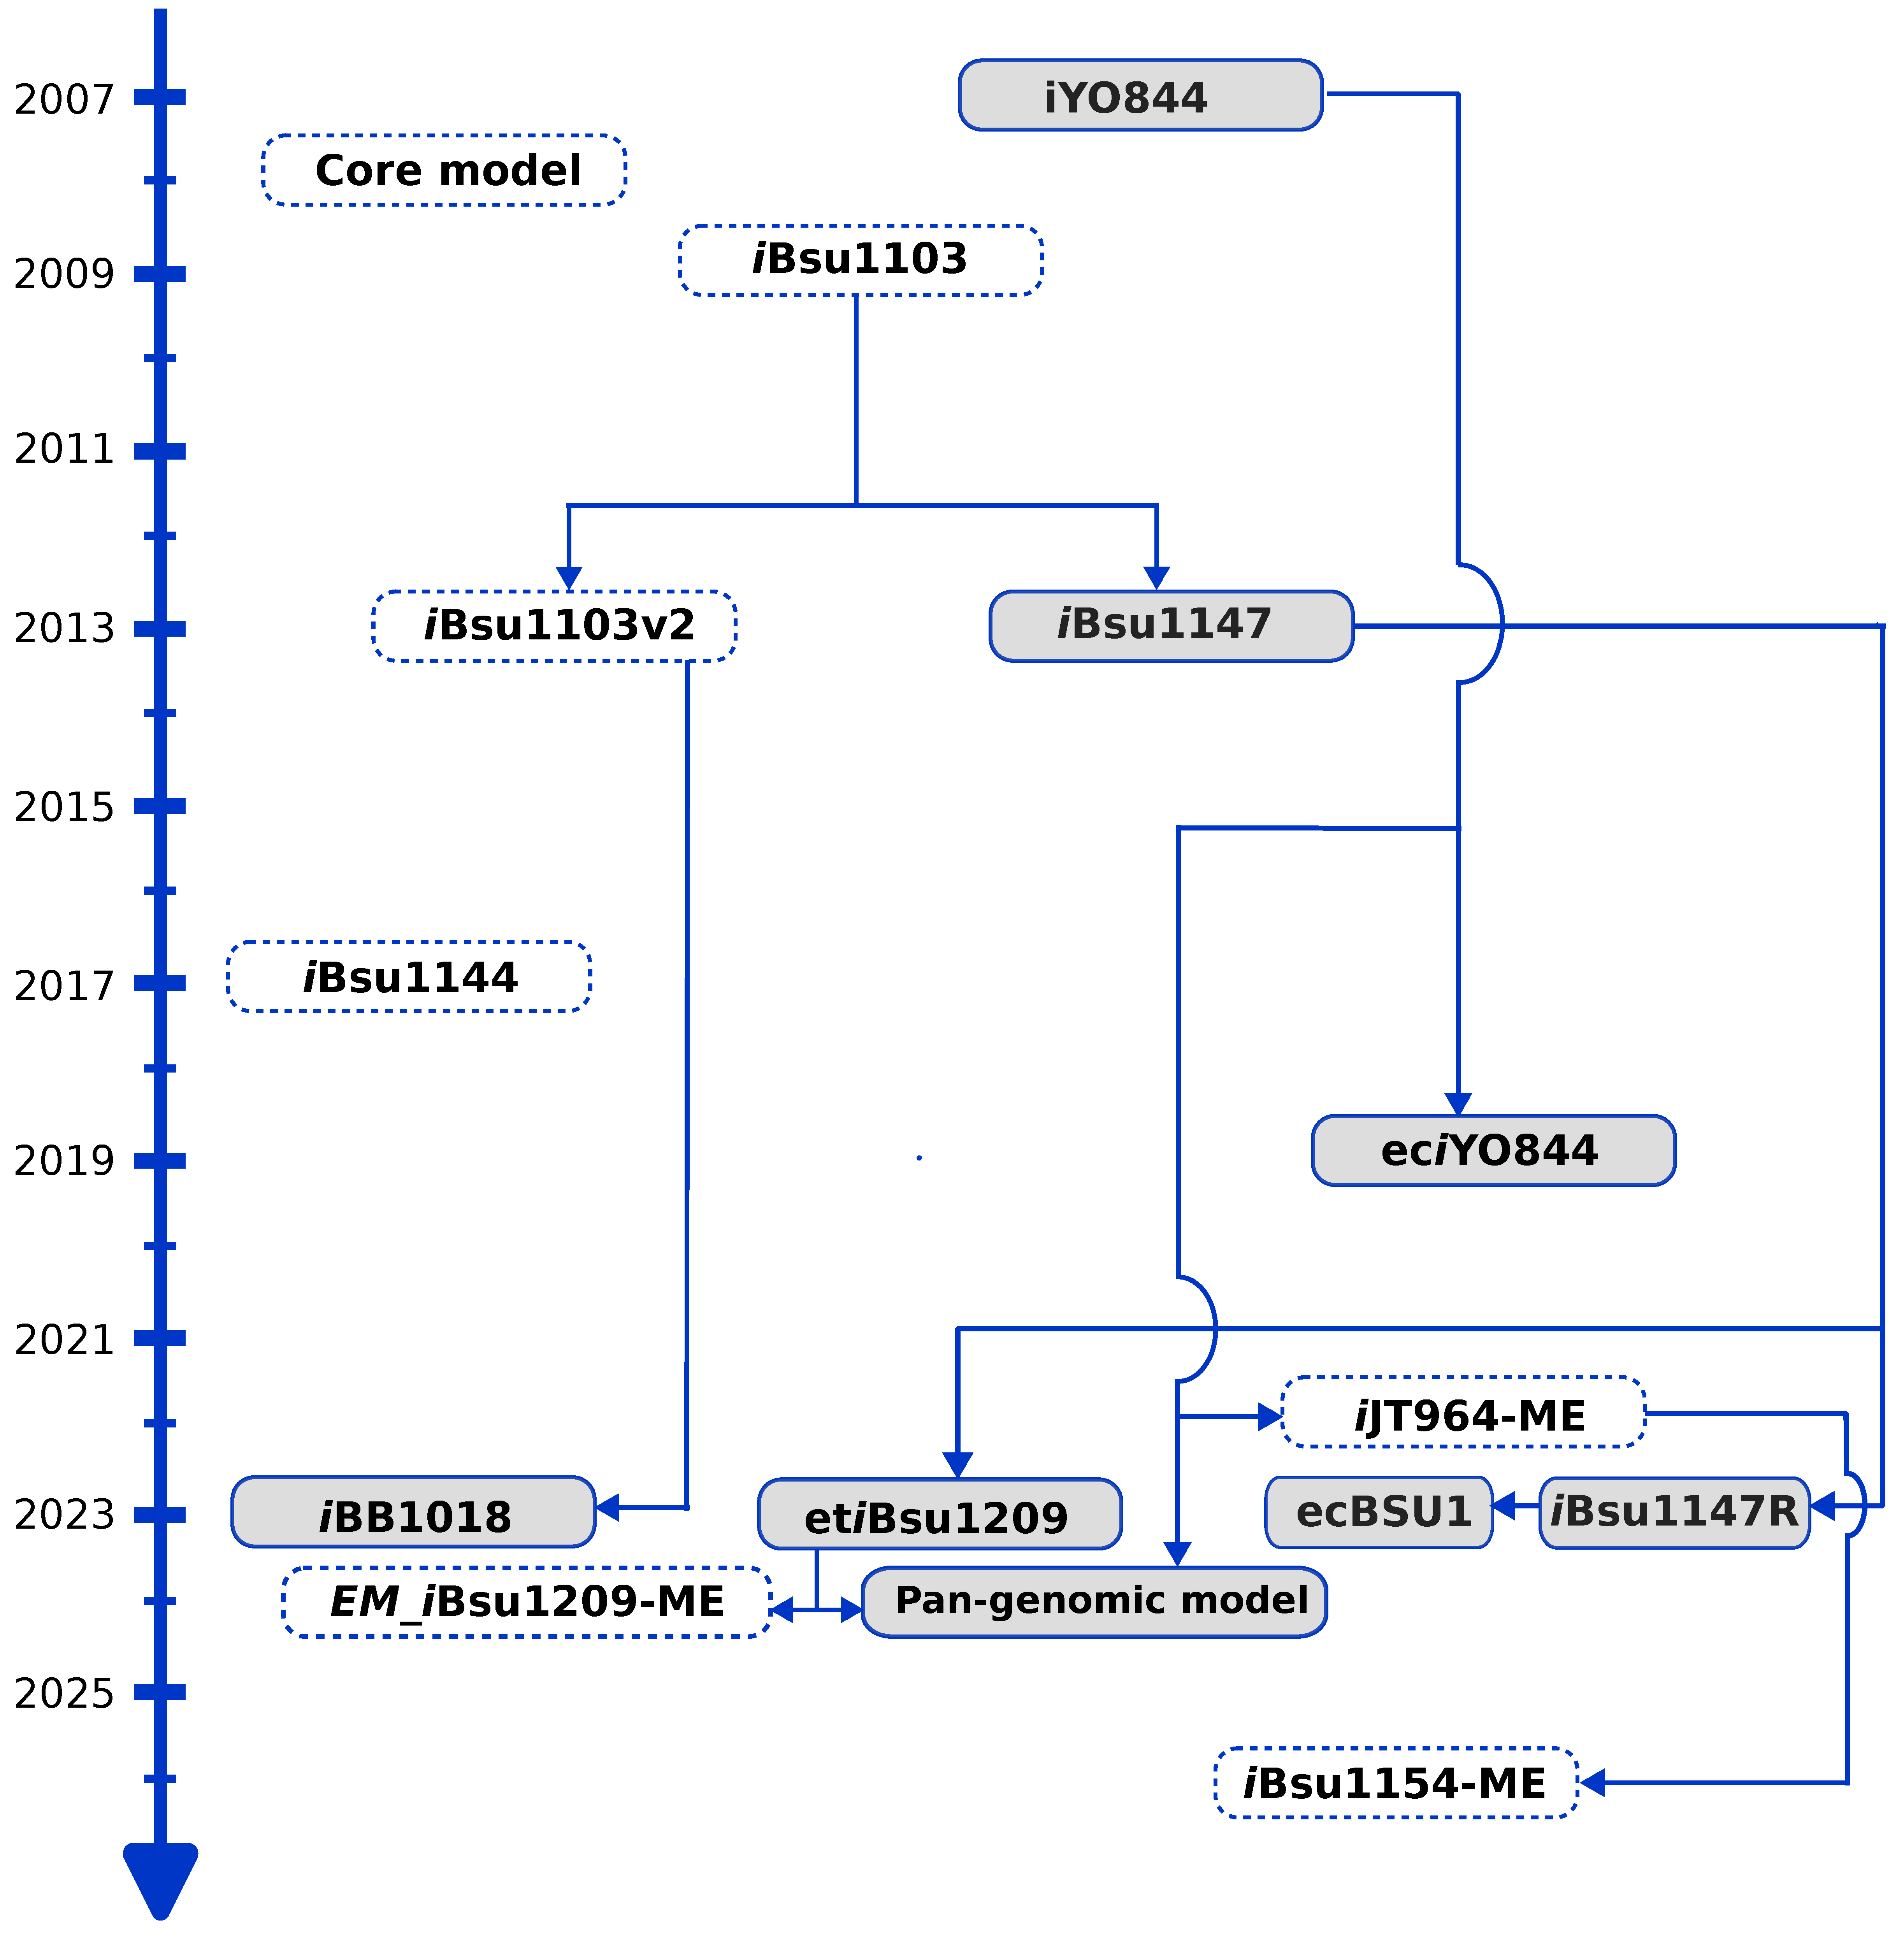
\includegraphics[width=0.8\linewidth]{figures/Timeline.pdf}
    \caption{GEM timeline evolution for \textit{B. subtilis}. Models in discontinuous boxes were not assessed in this study.}
    \label{fig:evolution}
\end{figure}


\section{Methods}

\subsection{Flux Balance Analysis framework}

Every simulation reported in this work rests on Flux Balance Analysis (FBA), a constraint-based method that predicts metabolic phenotypes from a GEM without requiring kinetic parameters \parencite{henao-2020}. The network is encoded in a stoichiometric matrix $S \in \mathbb{R}^{m \times n}$, whose element $S_{ij}$ is the coefficient of metabolite $i$ in reaction $j$, for $m$ metabolites and $n$ reactions. Two constraints delimit the space of admissible flux vectors $v$: the pseudo-steady-state assumption, under which internal metabolite concentrations do not change over time and production must balance consumption ($Sv = 0$); and lower and upper bounds on each flux ($l \leq v \leq u$), which encode reaction reversibility, thermodynamic feasibility and the uptake and secretion rates imposed by the simulated medium \parencite{orth-2010}.

Because genome-scale networks are underdetermined, this feasible space contains infinitely many flux distributions. FBA selects one by maximizing a biologically meaningful linear objective, here the biomass synthesis reaction as a proxy for growth, which casts the problem as a linear program:

\begin{equation}
\begin{aligned}
\max_{v} \; Z = c^{T}v \\
\text{subject to} \quad
& Sv = 0, \\
& l \leq v \leq u,
\end{aligned}
\label{eq:fba}
\end{equation}

where $c$ is the objective coefficient vector selecting the biomass reaction and $Z$ the optimal objective value, interpreted as the predicted specific growth rate. Solving \autoref{eq:fba} therefore returns both a growth rate and an intracellular flux distribution consistent with the environmental conditions imposed through $l$ and $u$ \parencites{pinzon-2018}{orth-2010}. Unless otherwise stated, those conditions were M9 minimal medium (Table S1) with glucose as the carbon source. This formulation underlies the growth-rate reproduction, glucose-uptake scanning, gene essentiality and carbon-source utilization analyses.

The optimal growth rate, however, does not fix the flux distribution uniquely: isozymes, alternative routes and reversible reaction pairs allow many distributions to reach the same $Z$. Where the flux distribution itself was the read-out rather than the objective value, we used parsimonious FBA (pFBA), which adds a second optimization on top of \autoref{eq:fba}. Once the optimal growth rate $Z^{*}$ has been obtained, total flux is minimized while that growth rate is held fixed:

\begin{equation}
\begin{aligned}
\min \sum_{i=1}^{n} |v_i| \\
\text{subject to} \quad
& Sv = 0, \\
& l \leq v \leq u, \\
& c^{T}v = Z^{*}.
\end{aligned}
\end{equation}

Under the assumption that cells minimize the enzymatic investment needed to sustain a given growth rate, this second step eliminates futile cycles and arbitrary flux through redundant pathways, yielding a single reproducible flux distribution \parencite{holzhutter-2004}.

\subsection{Model compilation and processing}
We compiled the models from different sources and formats listed in \autoref{tab:model_compilation}. The Systems Biology Markup Language (SBML) was selected as the target format. The core model and iBsu1144 were not converted due to their outdated format, eciYO844, etiBsu1209 and the pangenomic model were converted to SBML using the COBRA Toolbox v3.0 in MATLAB. The submodel for \textit{Bacillus subtilis} 168 was generated from the pangenomic model following its reconstruction procedure \parencite{neal-2024}. On the other hand, ecBSU1 and iBsu1147R JSON models were converted using COBRApy’s "write\_sbml\_model" function \parencite{ebrahim-2013}. 


\begin{table}[H]
\centering
\caption{Genome-scale metabolic models of \textit{Bacillus subtilis} compiled for this study. ME-models were not included, as their analysis workflow differs substantially.}
\label{tab:model_compilation}
\begin{tabular}{lll}
\hline
\textbf{Model} & \textbf{Original Format} & \textbf{Source} \\
\hline
iYO844 & SBML & BiGG Models \\
Core model & Excel & Supplementary material \\
iBsu1103 & SBML & BioModels \\
iBsu1103v2 & SBML & Supplementary material \\
iBsu1147 & SBML & Supplementary material \\
iBsu1144 & Excel & Author communication \\
eciYO844 & MATLAB & Supplementary material \\
etiBsu1209 & MATLAB & Author communication \\
iBB1018 & SBML & Supplementary material \\
iBsu1147R & JSON & GitHub repository \\
ecBSU1 & JSON & GitHub repository \\
Pan-genome model & MATLAB & GitHub repository \\
\hline
\end{tabular}
\end{table}

Nomenclature unification across all models was necessary. All identifiers were thus standardized to the BiGG model naming system \parencite{king-2015}. This was performed using the Python library mergem \parencite{hari-2024}, which allows automated translation of metabolite and reaction identifiers across databases. When needed, additional unification steps were done like converting eciYO844's BSubCyc gene nomenclature to locus tags and mapping reaction IDs missing from the mergem translation. 
Then, GEMs were annotated with Systems Biology Ontology (SBO) terms using the online tool SBOannotator \parencite{leonidou-2023}, which classifies model components based on their biological roles and functions. Final and annotated models were then validated with libSBML checks \parencite{bornstein-2008}.

\subsection{Structural count, quality scores and SBO classification}
To identify the amount of genes, metabolites and reactions actually present in the three metabolic reconstructions the Python function "len" was used which returned the length of each of these metabolic objects.  
Model quality was then evaluated using the standard Metabolic Model Testing tool memote, which executes a suite of structural and functional tests and assigns a quality score to each model \parencite{lieven-2020}. Also, reactions were classified based on their SBO terms.
The core model and iBSu1144 were excluded starting from this analysis and were not considered in any subsequent steps, due to their outdated and incompatible formats. ME-models were also excluded, as their workflow analysis differs significantly. Finally, iBsu1103, iBsu1103v2, and iBsu1209 were not included in the following analyses because they produced infeasible growth predictions.

\subsection{Reproduction of literature \textit{in silico} experiments}
Three \textit{in vitro} experiments, previously used to validate \textit{B. subtilis} GEMs were employed to assess the accuracy of the selected model predictions. The first set of experimental data was based on the uptake and growth rates reported for different carbon sources i.e. glucose, glycerol, gluconate, malate, pyruvate, fructose and the mix of glucose and malate and the mix of succinate and glutamate \parencite{chubukov-2013}. The second experimental data reported the growth rates in chemostat fermentations in which the import flux was also measured using as carbon sources glucose and mixes of glucose with acetoin, gluconate, citrate or acetate \parencite{dauner-2001C}. For both experiments, the default glucose exchange bound (EX\_glc\_\_D\_e) was closed before applying each condition's reported import flux(es) as reaction lower bounds.
While the third experimental data corresponds to the knock out of the cytochrome caa$_3$ oxidase reaction (CYOO3) applied to the same conditions of the second experimental set. Since reported literature points that this knock out could improve predictions \parencite{oh-2007}. 
In addition to these three condition-matched experiments, phenotype phase planes were constructed for each model by scanning the glucose and oxygen exchange bounds from 0 to \(-15\) and \(-30\ \mathrm{mmol\ gDW^{-1}\ h^{-1}}\) respectively over a grid, holding all other medium bounds at their M9 values, and recording the optimal growth rate at each node \parencite{edwards-2001}.

To evaluate predictive performance, simulated growth rates were compared against the experimentally measured values under all tested conditions. Deviations for individual conditions are displayed as relative errors in the corresponding heatmaps, while each model's performance over a whole experiment was summarized using Lin's concordance correlation coefficient (CCC) \parencite{lin-1989},

\begin{equation}
\text{CCC} = \frac{2\,r\,\sigma_{sim}\,\sigma_{exp}}{\sigma_{sim}^{2} + \sigma_{exp}^{2} + (\bar{\mu}_{sim} - \bar{\mu}_{exp})^{2}}
\label{eq:ccc}
\end{equation}

where $r$ is Pearson's correlation coefficient between predicted and measured growth rates, $\sigma$ their standard deviations and $\bar{\mu}$ their means. CCC measures agreement with the identity line penalizing a systematic offset and a difference in scale respectively. Root mean square error (RMSE), mean absolute error (MAE) and bias (the mean signed deviation) were computed alongside it. 

\subsection{Gene essentiality analysis}
Gene essentiality analysis was performed on six of the seven models retained for functional simulations (iYO844, iBsu1147, eciYO844, iBB1018, iBsu1147R and ecBSU1); the pangenome-derived Submodel was excluded from this analysis because its gene IDs could not be mapped to locus tags.
To identify the set of essential genes for each GEM, the \textit{COBRApy} function "find\_essential\_genes" \parencite{ebrahim-2013} was employed.
This function returns an array containing the loci of essential genes, defined as those whose deletion results in a simulated growth rate below \(10^{-3}\ \mathrm{h}^{-1}\).
Predicted gene identifiers were matched to the experimentally determined list of essential genes reported by \parencite{kobayashi-2003} by locus tag. Based on this comparison, a confusion matrix was generated to evaluate each model’s performance in classifying genes as essential or non-essential.
Thus, genes correctly predicted as essential were defined as True Positives (TP), while essential genes incorrectly predicted as non-essential were False Negatives (FN). Conversely, non-essential genes correctly identified as such were True Negatives (TN), and non-essential genes misclassified as essential were False Positives (FP).

The predictive accuracy of each model was then assessed using several metrics \parencite{tibocha-bonilla-2022}: Recall, Specificity, False Discovery Rate, Precision, Accuracy, F1 Score, Matthews Correlation Coefficient (MCC), and coverage. These metrics were calculated according to the following definitions:

Recall: proportion of essential genes correctly identified.
\begin{equation}
\text{Recall} = \frac{TP}{TP + FN}
\label{eq:1}
\end{equation}

Specificity: proportion of non-essential genes correctly identified.
\begin{equation}
\text{Specificity} = \frac{TN}{TN + FP}
\end{equation}

False Discovery Rate (FDR): proportion of genes predicted to be essential that are not actually essential.
\begin{equation}
\text{FDR} = \frac{FP}{TP + FP}
\end{equation}

Precision: proportion of correct essentiality predictions.
\begin{equation}
\text{Precision} = \frac{TP}{TP + FP}
\end{equation}

Accuracy: proportion of all genes correctly classified, essential or not.
\begin{equation}
\text{Accuracy} = \frac{TP + TN}{TP + TN + FP + FN}
\end{equation}

F1 Score: harmonic mean of Precision and Recall.
\begin{equation}
F1 = \frac{2 \cdot \text{Precision} \cdot \text{Recall}}{\text{Precision} + \text{Recall}}
\end{equation}

Matthews Correlation Coefficient (MCC): robust overall measure of classifier performance, considering all cases (TP, TN, FP, FN).
\begin{equation}
\text{MCC} = 
\frac{(TP \cdot TN) - (FP \cdot FN)}
{\sqrt{(TP + FP)(TP + FN)(TN + FP)(TN + FN)}}
\end{equation}

Coverage: portion of the genome covered by the model.
\begin{equation}
\text{Coverage} = \frac{\text{genes in model}}{\text{total genes}}
\label{eq:6}
\end{equation}

\subsection{Central carbon metabolism flux distribution analysis}
Intracellular flux distributions were compared, across the same seven models, for 28 reactions spanning glycolysis (EMP pathway), the TCA cycle and the pentose phosphate pathway (PPP), against the corresponding experimental fluxes reported by \parencite{chubukov-2013}. Simulations were run under M9 minimal medium with the glucose uptake bound fixed at \(-7.63\ \mathrm{mmol\ gDW^{-1}\ h^{-1}}\) to match the experimental condition. Fluxes were resolved with parsimonious FBA (pFBA) rather than plain FBA. ecBSU1 had reactions represented as duplicated isozymes or as separate forward/reverse half-reactions, its net flux was computed as the sum of forward minus reverse fluxes across all corresponding instances.

Agreement with the measured fluxes was quantified with the same concordance correlation coefficient used for the growth rates (\autoref{eq:ccc}), together with a normalized root mean square error (NRMSE), MAE and bias.

\subsection{Biolog carbon-source utilization analysis}
Predicted carbon-source utilization phenotypes were compared against high-throughput Biolog phenotyping data \parencite{oh-2007} for the seven models retained for functional simulations. For each model, every carbon-containing exchange reaction was closed, and each experimental carbon source's exchange reaction was then opened individually as the sole carbon source, at an uptake rate of \(-7.5\ \mathrm{mmol\ gDW^{-1}\ h^{-1}}\). Growth was called positive when FBA returned an objective value at or above the \(10^{-3}\ \mathrm{h}^{-1}\) threshold also used for gene essentiality. Predictions were compared against the corresponding qualitative Biolog call (growth/no growth). Carbon sources whose exchange reaction could not be resolved in a given model were reported as untested rather than as a negative prediction.


\subsection{Software and code availability}

All analyses were implemented in Python. Constraint-based simulations were performed with COBRApy 0.29.1 \parencite{ebrahim-2013} using Gurobi as the linear programming solver. Model standardization and curation used mergem 1.1.0 for identifier translation to BiGG nomenclature \parencite{hari-2024}, SBOannotator 3.0.4 for SBO term assignment \parencite{leonidou-2023}, libSBML 5.20.5 for validation, and MEMOTE 0.17.0 for quality scoring \parencite{lieven-2020}. Format conversions that could not be handled in Python were performed in MATLAB with the COBRA Toolbox v3.0 \parencite{heirendt-2019}. 

All models, datasets, analysis code and manuscript sources are openly available at \url{https://github.com/felipeg210303/Bacillus_GEMs_Paper}, together with a conda environment specification pinning every dependency. The repository provides each model at three stages: as originally obtained, standardized to SBML with BiGG nomenclature, and SBO-annotated, so that the effect of the preprocessing can be traced, and the analyses are organized as a numbered sequence of notebooks that regenerate every figure and table presented here from those inputs.


\section{Results}

\subsection{Model features and quality scores}
An initial evaluation of the selected GEMs was based on the number of genes, metabolites and reactions reported for each one. The ecBSU1 model exhibits the highest number of reactions among all evaluated models (3307), due to the presence of duplicated reactions (\autoref{fig:structural}). In general, all models show a higher number of reactions than metabolites, and more metabolites than genes, with the exception of the pangenomic model, which deviates from this pattern showing more genes followed by the number of reactions and the number of metabolites (\autoref{fig:structural}).
We thus assessed the model quality by MEMOTE score (\autoref{fig:structural}A). iYO844 and iBsu1103 achieved the highest scores (82.48\% and 73.86\%, respectively), followed by iBB1018 (64.72\%). On the other hand, iBsu1209 had the lowest score (47.88\%), and the pangenomic model did not return a score, indicating potential compatibility issues.
The gene counts require a further qualification. Although the pangenome-derived Submodel contains more genes than any other reconstruction (2364), 1756 of them carry no gene--protein--reaction association (Table S2) and therefore cannot participate in any simulation; the same absence is what prevented this model from being included in the gene essentiality analysis. Its apparent advantage in genomic coverage is thus largely nominal.

The three models excluded from the functional analyses failed for identifiable reasons. iBsu1103 and iBsu1103v2 returned growth rates above 200~h$^{-1}$ because none of the 31 metabolites of their biomass reaction carries a chemical formula, so the reaction is not mass-balanced and can be satisfied at negligible cost. iBsu1209, whose biomass metabolites are fully specified, returned no growth under any condition instead.

Regarding the SBO distribution, iBsu1209 showed an abnormal pattern with only biochemical and phosphorylation reactions.
Notably, eciYO844 and the pangenomic model had zero reactions annotated with SBO terms related to transport reactions.
\begin{figure} [H]
    \centering  
    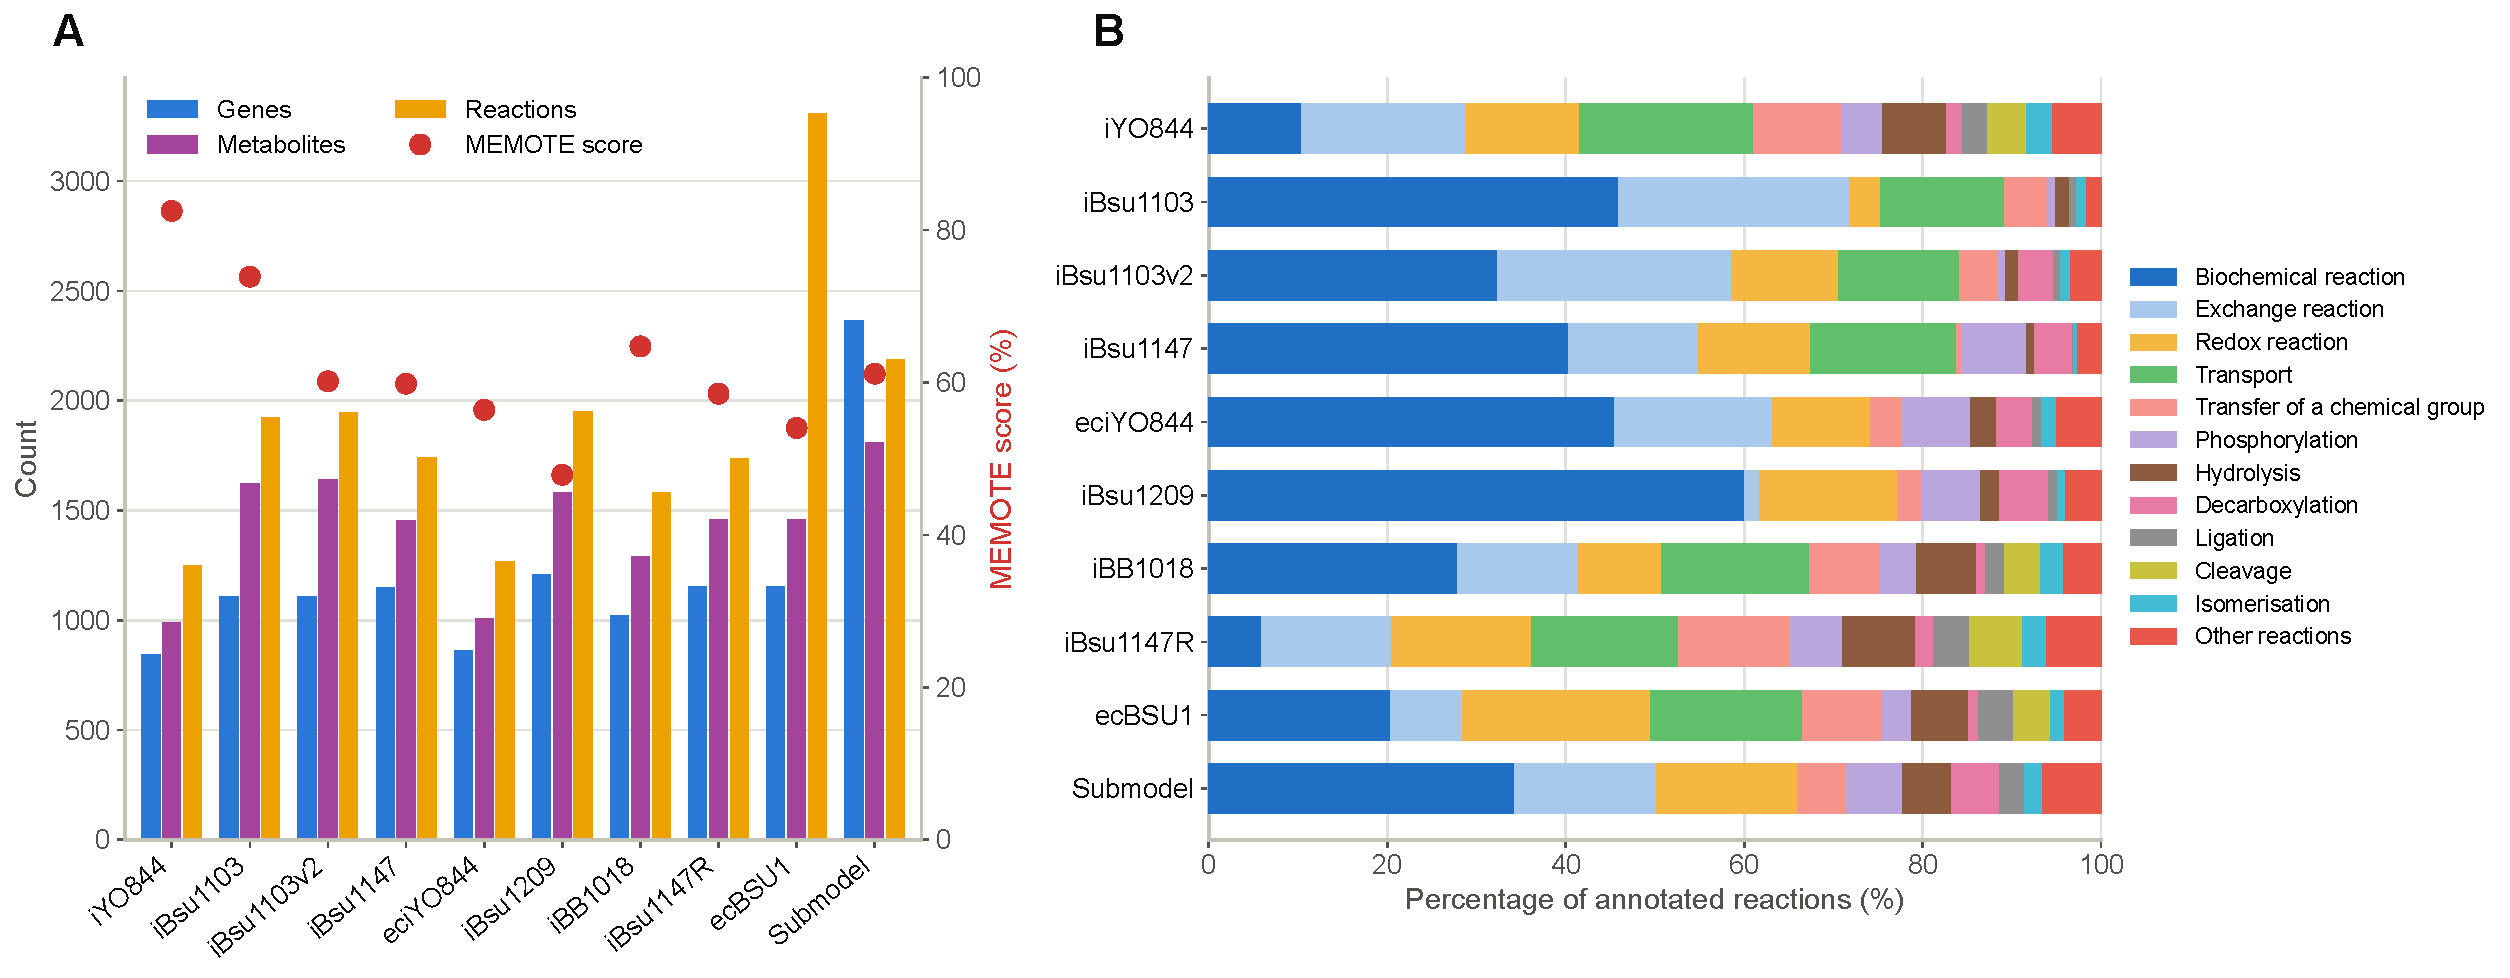
\includegraphics[width=\linewidth]{../analysis/results/figures/Fig_features_SBO.pdf}
    \caption{Structural composition and annotation of the evaluated GEMs. \textbf{A.} Number of genes, metabolites and reactions per model (bars, left axis) and MEMOTE score (points, right axis). \textbf{B.} Distribution of reactions by SBO term, as a percentage of the annotated reactions of each model. Transport-related terms are pooled into a single category and the remaining terms are grouped as other reactions.}
    \label{fig:structural}
\end{figure}

\subsection{\textit{In silico} versus \textit{in vitro} growth rates}

Two experimental datasets, spanning three simulated experiments, were reproduced and compared against measured growth rates \parencite{chubukov-2013, dauner-2001C}. Models returning unrealistic growth rates (iBsu1103, iBsu1103v2 and iBsu1209) were excluded from these and all subsequent analyses.

Hierarchical clustering of the relative errors grouped iYO844, iBB1018 and iBsu1147R together in all three experiments, indicating similar predictive behaviour despite differences in model size and reconstruction history (\autoref{fig:clustermap}A--C). eciYO844 clustered close to these manually curated reconstructions, whereas ecBSU1 formed a separate branch.

In the first experiment, eciYO844 did not predict growth under any glucose-free condition and iBsu1147 returned no feasible solution on malate as the sole carbon source. All models overestimated growth on pyruvate, and all underestimated it on glycerol and on the malate--glucose mixture. Concordance correlation coefficients ranged from 0.33 for eciYO844, whose failure to grow on six of the eight substrates dominates its score, to 0.91 for iBB1018.

In the second experiment, every model overestimated growth under every condition, and increasingly so at higher glucose uptake rates. This behaviour has been attributed to the preferential routing of electron transport through the cytochrome caa$_3$ oxidase, which yields more ATP than the alternative oxidases but is repressed during growth on glucose \parencite{oh-2007}. Deleting this reaction in the third experiment reduced the relative error under nearly all conditions and raised the concordance correlation coefficient from 0.79--0.89 to 0.96--0.98, consistent with unrestricted respiratory flux being the principal source of the overestimation. The exception was iBsu1147, whose predictions were numerically identical before and after the deletion. The reaction is present in that model but carries no flux at the optimum, respiration running entirely through the \textit{aa}$_3$-600 quinol oxidase, which translocates four protons per oxygen atom reduced against seven for the cytochrome \textit{c} branch. iBsu1147 therefore already respires through the lower-yielding route that the deletion is intended to impose on the other models, and its persistent overestimation of growth must have a different origin.

Phenotype phase planes over glucose and oxygen uptake were largely comparable across models, with maximum growth rates between 0.55 and 0.63~h$^{-1}$ and oxygen-to-glucose ratios along the line of optimality between 2.1 and 2.8 (Figure S5). Every surface saturates well inside the range scanned, and relaxing each medium component in turn identified ammonia, capped at 5 mmol~gDW$^{-1}$~h$^{-1}$, rather than carbon or oxygen, as the constraint responsible in all seven models; lifting it more than doubled the attainable growth rate. The plateau is therefore a property of the defined medium rather than of the reconstructions, and comparisons at high substrate supply should be read accordingly. The one exception is eciYO844, which saturates at 0.68~h$^{-1}$ with every medium bound released, its ceiling being set by its own enzyme capacity constraints. The models also differed in how much oxygen was required before growth began, eciYO844 again requiring twice as much as any other.
\begin{figure} [H]
    \centering
    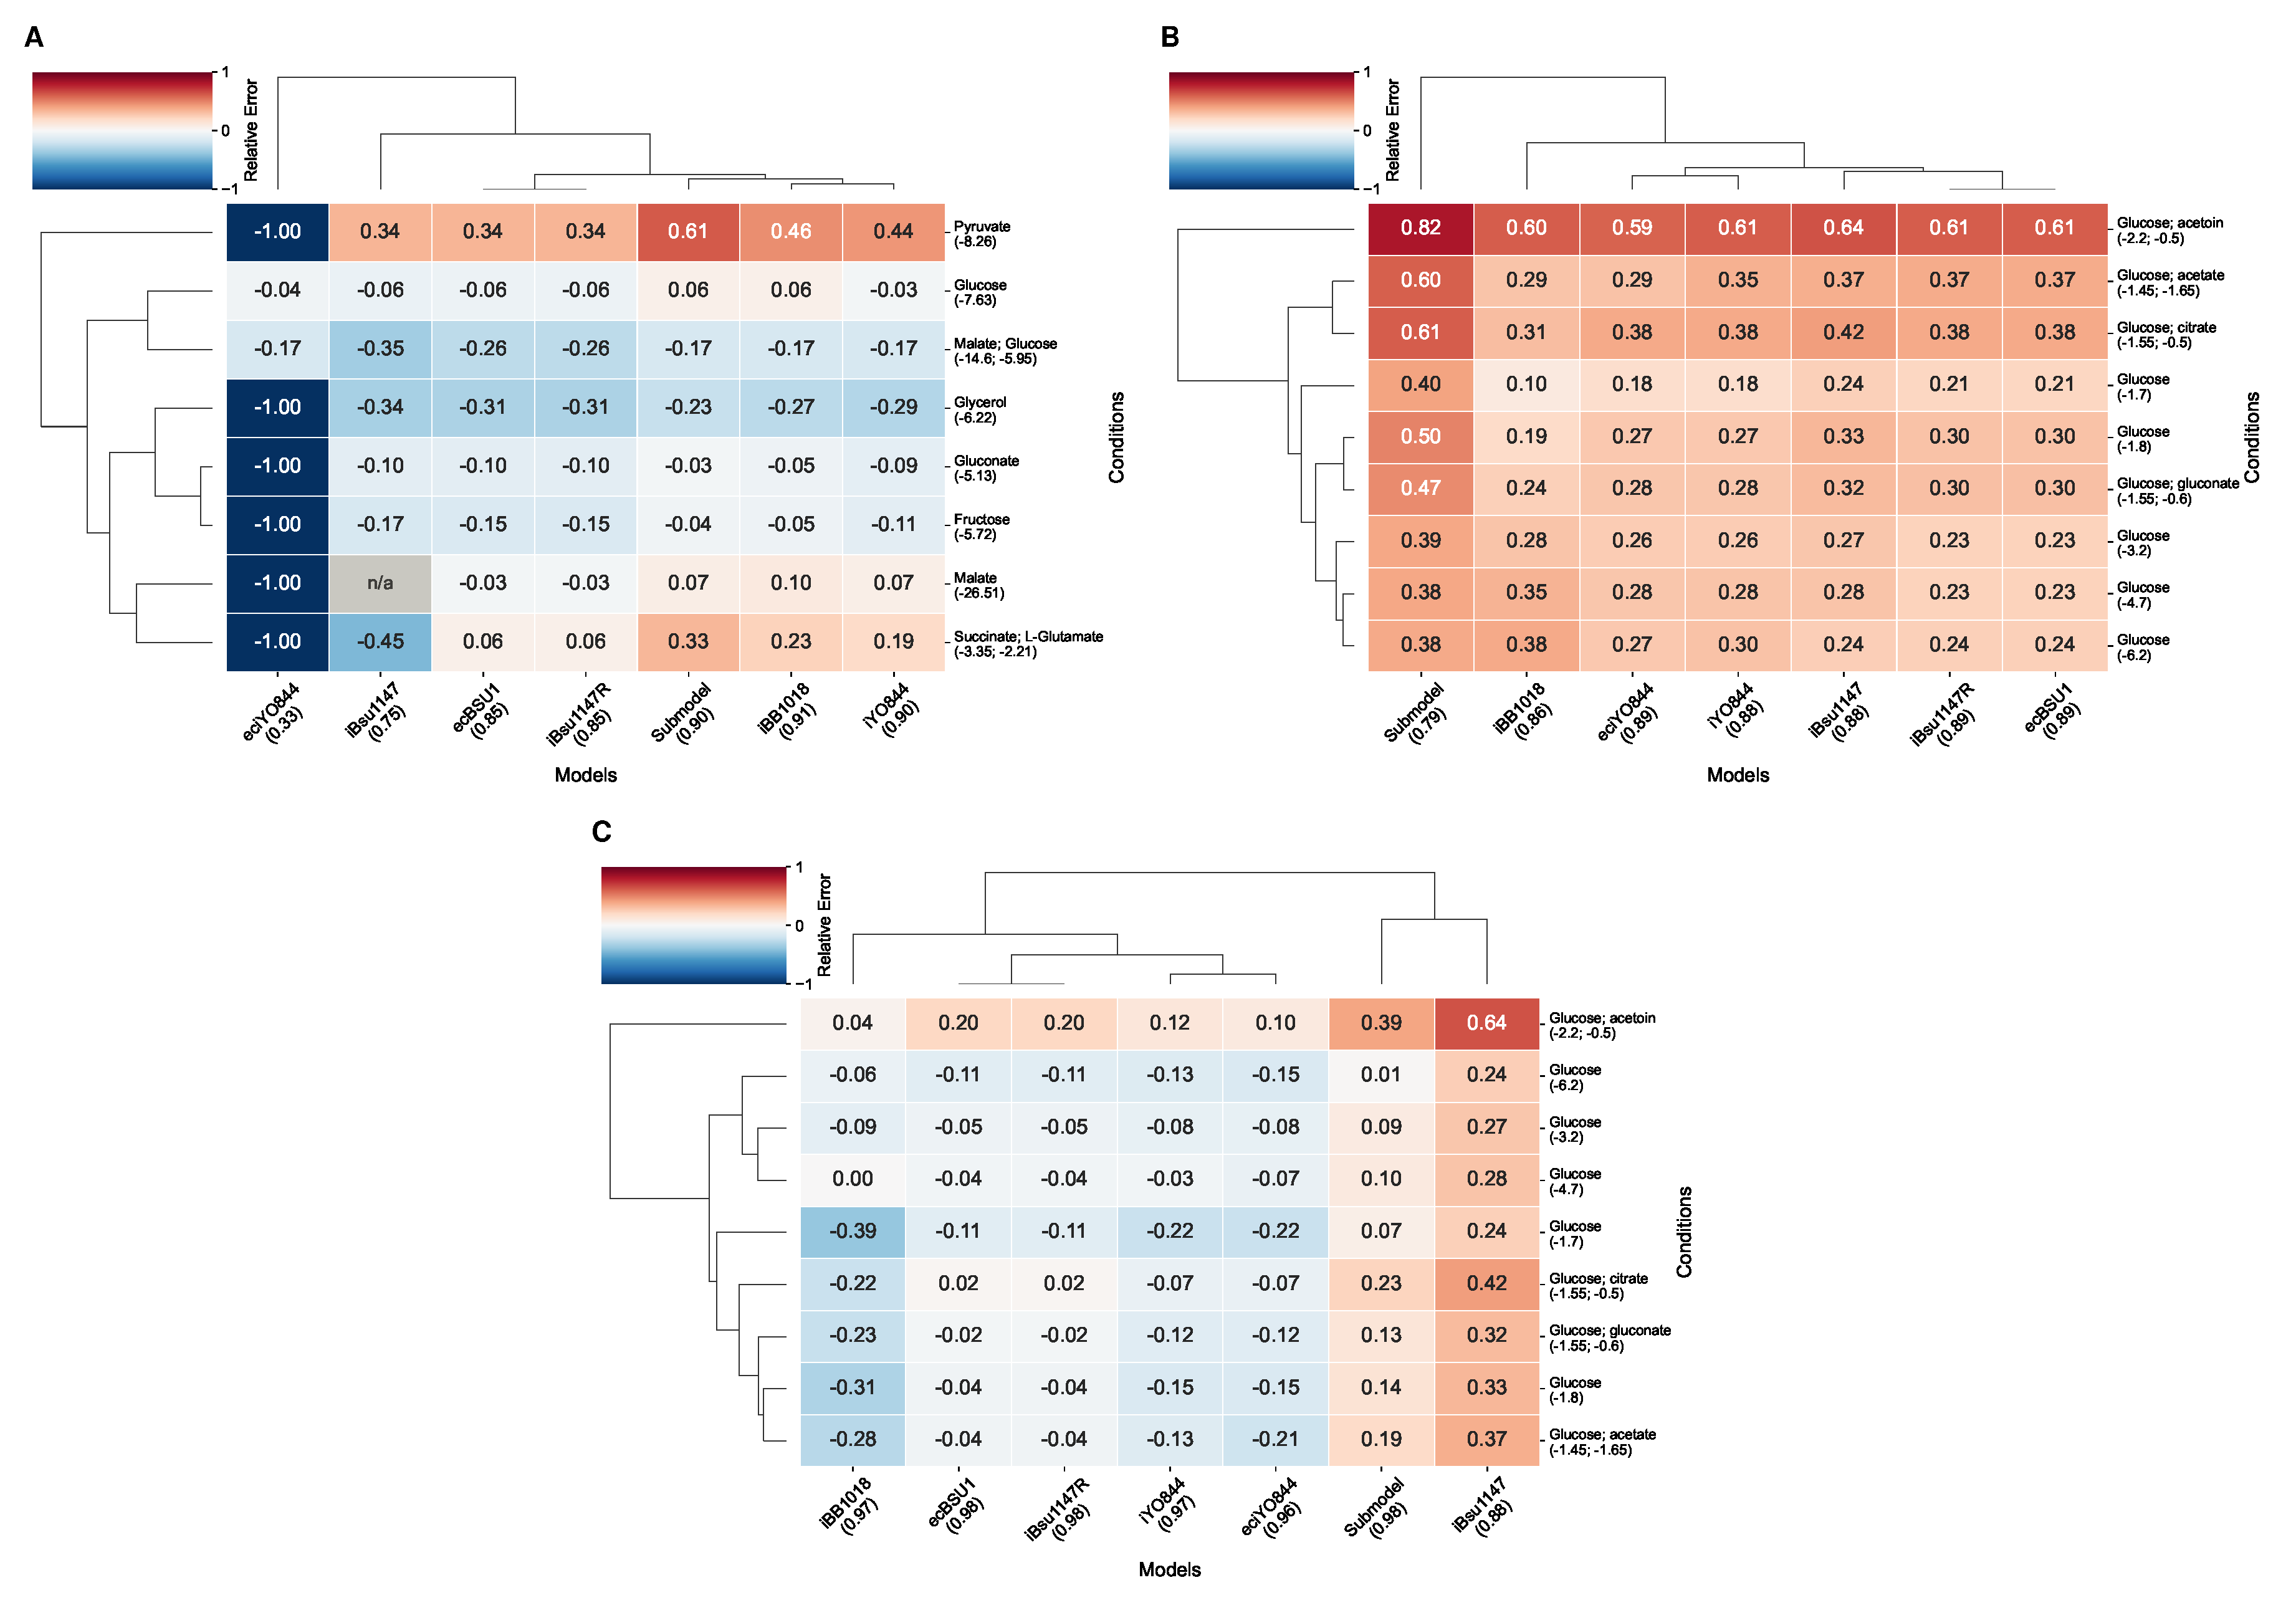
\includegraphics[width=\linewidth]{../analysis/results/figures/Fig_growth_composite.pdf}
    \caption{Relative error of predicted growth rates per condition, clustered by model and by condition; blue denotes underestimation and red overestimation. Values in parentheses below each model give its concordance correlation coefficient for that experiment, and those beside each condition give the imposed import fluxes in mmol~gDW$^{-1}$~h$^{-1}$. n/a: no feasible solution. \textbf{A.} Carbon sources \parencite{chubukov-2013}. \textbf{B.} Glucose and glucose-containing mixtures \parencite{dauner-2001C}. \textbf{C.} As in B, after deletion of the cytochrome caa$_3$ oxidase reaction.}
    \label{fig:clustermap}
\end{figure}

\subsection{Gene essentiality analysis}

Predicted essential genes were compared against the experimentally determined set \parencite{kobayashi-2003} for the six models whose gene identifiers could be mapped to locus tags (\autoref{fig:gene_essentiality}). Ranked by Matthews correlation coefficient, iBsu1147R and ecBSU1 performed best (0.62), followed by iBsu1147 (0.59) and iBB1018 (0.58), with iYO844 and eciYO844 last (0.46 each). The ordering broadly follows reconstruction size, the models carrying more genes recovering a larger part of the essential set.

All six models departed from the experimental data in the same direction. Recall ranged from 0.70 to 0.85, so most essential genes were identified, but precision reached only 0.42--0.58, indicating that between four and six of every ten genes predicted to be essential are experimentally dispensable. Specificity was uniformly high (0.86--0.88) and accuracy correspondingly so (0.84--0.87), although the latter reflects the composition of the dataset rather than predictive performance, since essential genes are outnumbered approximately eight to one and a model calling every gene non-essential would score about 0.85. Systematic overestimation of essentiality is an expected consequence of a purely stoichiometric formulation \parencite{bernstein-2023} \parencite{bernstein-2023}, in which the deletion of any gene that blocks a biomass precursor is lethal and no isoenzyme regulation, substrate promiscuity or metabolic rerouting is available to compensate.

Coverage further constrains the interpretation of these metrics. None of the models span more than 27\% of the 4332 genes of the experimental dataset (iBsu1147R and ecBSU1, 0.27; iYO844 and eciYO844, 0.19--0.20), so the values describe only the fraction of the genome each reconstruction represents.

\begin{figure} [H]
    \centering
    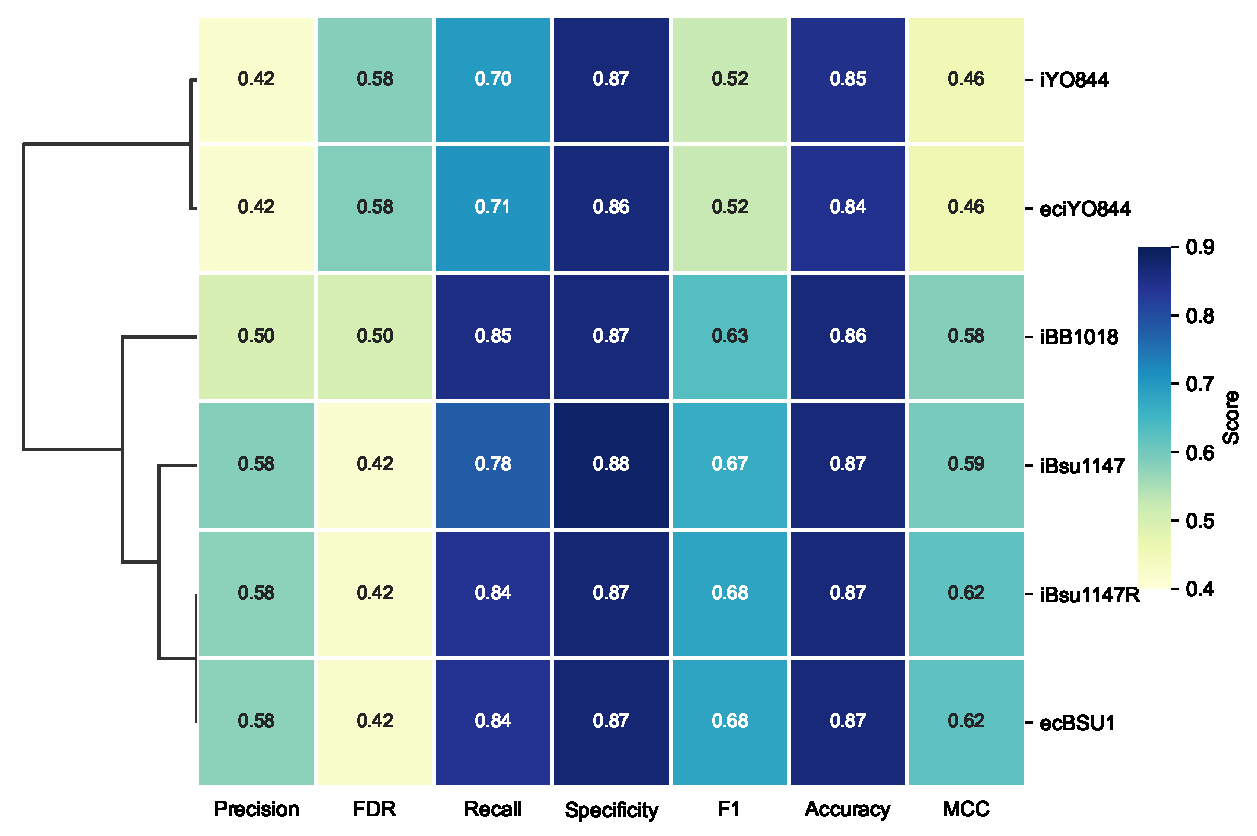
\includegraphics[width=0.9\linewidth]{../analysis/results/figures/Plot_GeneEssentiality_metrics_comparison.pdf}
    \caption{Gene essentiality prediction metrics per model, derived from confusion matrices of predicted against experimentally determined essentiality. Models are hierarchically clustered by their metric profile; metric columns are kept in a fixed order. Per-model confusion matrices are given in Figure S1.}
    \label{fig:gene_essentiality}
\end{figure}

\subsection{Fluxes across central carbon metabolism}


\begin{figure}[H]
\centering
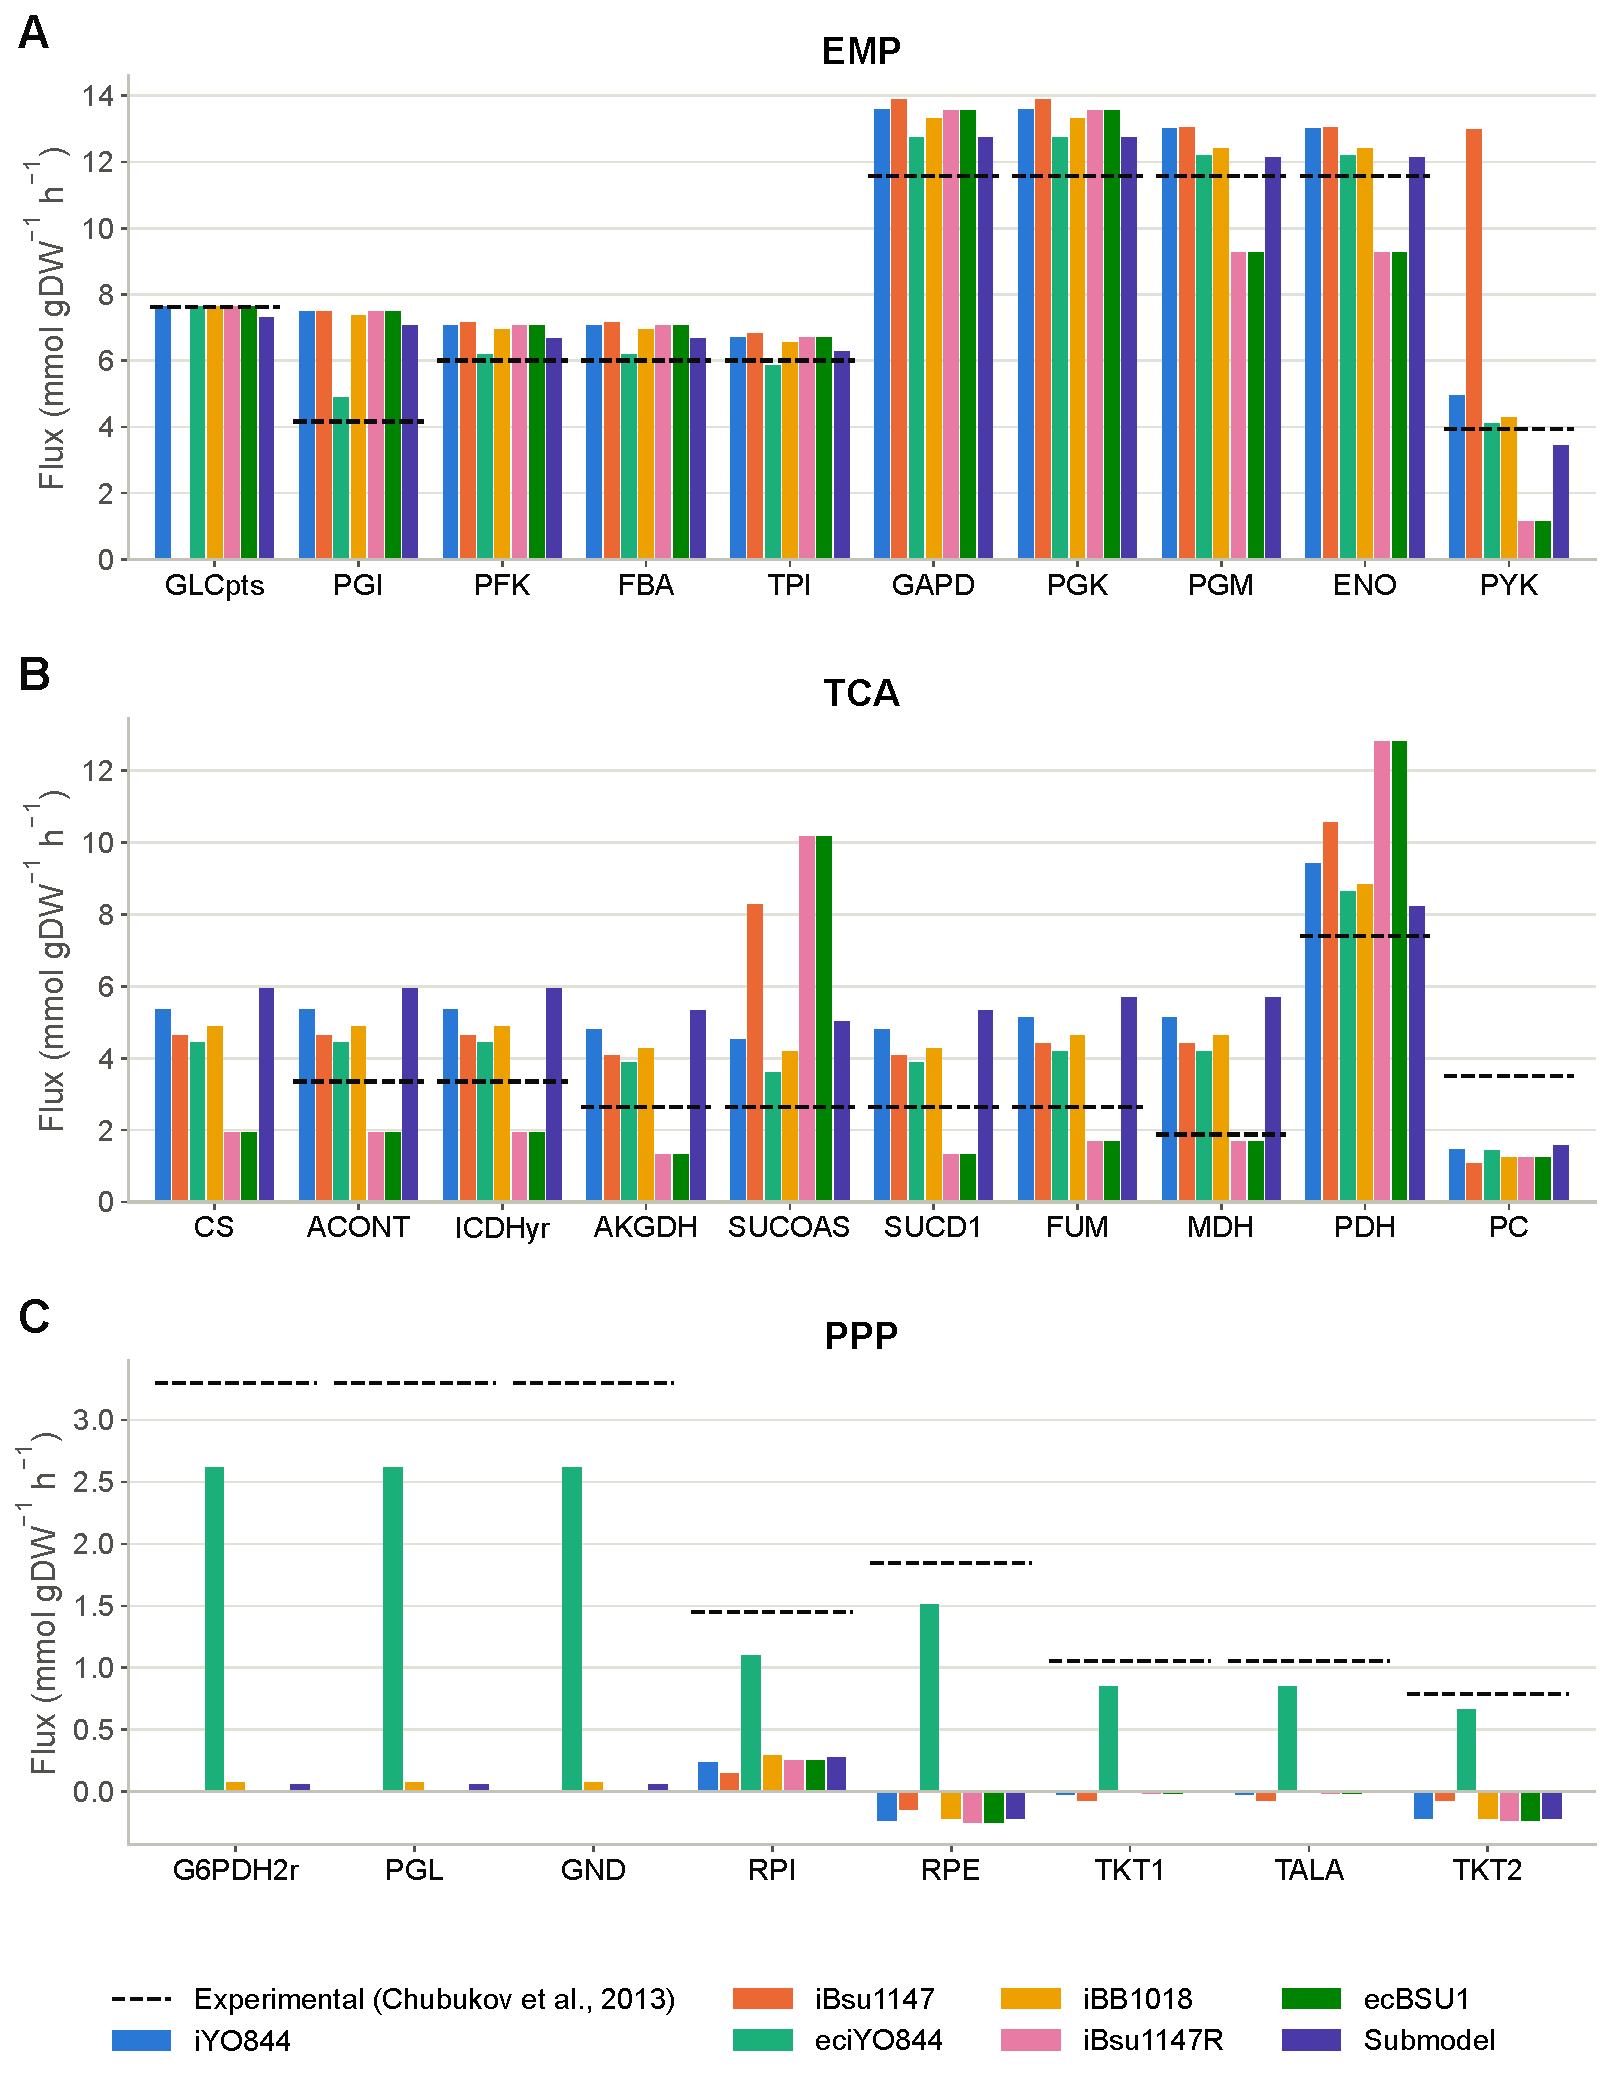
\includegraphics[width=0.95\textwidth]{../analysis/results/figures/carbon_metabolism_fluxes.pdf}
\caption{Intracellular flux distributions across central carbon metabolism, with the corresponding experimental fluxes shown as black ticks \parencite{chubukov-2013}. One panel per pathway, with one bar per model. Fluxes are expressed in the pathway-forward direction, so negative values denote flux in the opposite direction. }
\label{fig:carbon_metabolism_fluxes}
\end{figure}

Intracellular flux distributions were compared against measured fluxes across glycolysis, the TCA cycle and the pentose phosphate pathway (\autoref{fig:carbon_metabolism_fluxes}). Over the twenty independent reactions scored, eciYO844 reproduced the measured distribution most closely (CCC 0.95; normalized root mean square error 13.7\% of the glucose uptake rate), followed by iBB1018 (0.87), iYO844 (0.85), the Submodel (0.81), iBsu1147R and ecBSU1 (0.75) and iBsu1147 (0.71). The three magnitude-based statistics ranked the models identically, indicating that the ordering does not depend of the choice of statistic (Figure S3).

Agreement was unevenly distributed across pathways. Restricted to glycolysis, all models scored between 0.79 and 0.98; restricted to the TCA cycle, between 0.26 and 0.66; and restricted to the oxidative pentose phosphate pathway, six of the seven scored approximately 0.01. In those six models G6PDH2r, PGL and GND carried between 0 and 0.08 mmol~gDW$^{-1}$~h$^{-1}$ against a measured 3.30, and the non-oxidative steps ran in the reverse direction to supply the erythrose-4-phosphate and ribose-5-phosphate required for biomass. The branch is present in every reconstruction, so its inactivity reflects the optimization objective rather than a gap in the network: the NADPH demand is met at lower total flux through alternative routes, although the oxidative branch is the principal source of NADPH in glucose-grown cells \parencite{stincone-2015}. Only eciYO844 carried appreciable flux through the oxidative branch (2.61; CCC 0.89), and this difference accounts for most of its advantage. The same shortfall explains the one systematic discrepancy in glycolysis, where all models ran PGI at 7.0--7.5 against a measured 4.16, the approximately 3 mmol~gDW$^{-1}$~h$^{-1}$ diverted into the oxidative branch \textit{in vivo} remaining in the glycolytic trunk.

Two further deviations follow from specific features of the reconstructions. iBsu1147 overestimated pyruvate kinase threefold (12.99 against a measured 3.94), the largest single-reaction error in the comparison and the reason for its low glycolytic score (CCC 0.41); lacking a phosphotransferase system, this model must generate all of its pyruvate through PYK, whereas in the remaining models the PTS supplies most of it directly. Conversely, ecBSU1 and iBsu1147R underestimated the same reaction (1.14), their phosphoenolpyruvate being consumed by the PTS and by anaplerotic reactions. In three models the succinyl-CoA node was supplied mainly by acetoacetate:succinate CoA-transferase rather than by 2-oxoglutarate dehydrogenase, so that SUCOAS greatly exceeded AKGDH (ecBSU1, 11.3 against 0.1; iBsu1147R, 10.2 against 1.3; iBsu1147, 8.3 against 4.1) and the cycle was partly short-circuited.

ecBSU1 and iBsu1147R were indistinguishable under this condition, all 28 fluxes agreeing to within $2\times10^{-5}$ and both growing at 0.5546~h$^{-1}$. ecBSU1 is the enzyme-constrained build of iBsu1147R, but the SBML distribution used here carries no enzyme capacity bounds: of its 3307 reactions, only the ATP maintenance reaction and one exchange have a bound other than the default. The reaction splitting characteristic of the formulation is present, but the constraints that act on it are not, so under this representation the model is stoichiometrically equivalent to its parent.

\subsection{Carbon utilization analysis}

Qualitative growth predictions were compared against Biolog phenotyping data \parencite{oh-2007} for 96 carbon sources (\autoref{fig:carbon_utilization_heatmap}). By Matthews correlation coefficient, the pangenome-derived Submodel performed best (0.58), followed by iYO844 and iBB1018 (0.51 each), then iBsu1147R, ecBSU1 and eciYO844 (0.36), and finally iBsu1147 (0.26). Between 18 and 25 of the 96 substrates could not be tested in a given model because the corresponding exchange reaction was absent. The substrates that remained testable were strongly skewed towards growth, with six to eight positive calls for every negative one, since most substrates lacking an exchange reaction are ones the organism does not use; accuracy is therefore uninformative here, iBsu1147 reaching 0.82 while its Matthews correlation coefficient of 0.26 indicates performance close to chance.

The models departed from the experimental data in two opposite ways. iYO844, iBB1018 and the Submodel were permissive, recovering 89--91\% of the substrates supporting growth but correctly identifying only 67--80\% of those that do not, so that their errors were predominantly false positives. eciYO844 showed the converse behaviour, producing no false positives (specificity and precision of 1.00) but failing to predict growth on 30 of the 68 substrates that support it, giving a recall of 0.56. This is the same behaviour that prevented growth on six of the eight carbon sources of the first growth experiment, and it reflects the absence of the corresponding uptake reactions rather than an excess of constraint: releasing every enzyme capacity bound in the model leaves growth on those substrates at zero.

\begin{figure} [H]
    \centering
    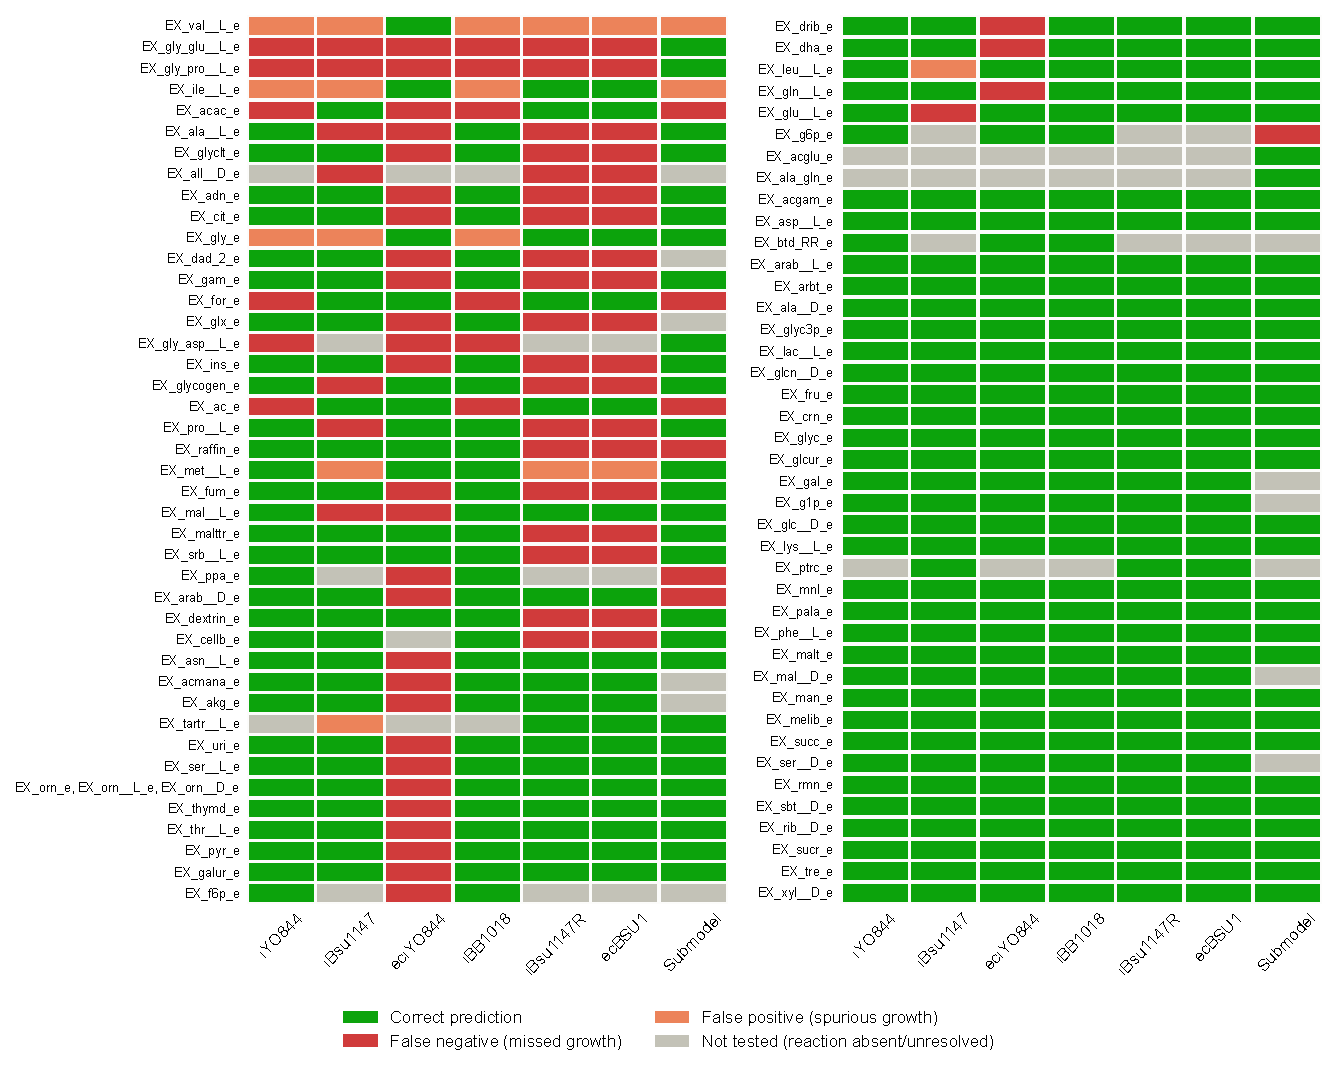
\includegraphics[width=1\linewidth]{../analysis/results/figures/Carbon_Utilization_Heatmap.pdf}
    \caption{Per-substrate carbon utilization predictions against experimental Biolog data \parencite{oh-2007}. Green, correct prediction; red, false negative; orange, false positive; grey, substrate not testable because the corresponding exchange reaction is absent from the model. Per-model confusion matrices are given in Figure S4.}
    \label{fig:carbon_utilization_heatmap}
\end{figure}

\subsection{Summary}

\begin{table}[H]
\centering
\footnotesize
\setlength{\tabcolsep}{4pt}
\caption{Summary of all tests applied in this study. Annotation depth is the proportion of reactions carrying an SBO term more specific than the generic ``biochemical reaction'' (SBO:0000176). CCC, concordance correlation coefficient; MCC, Matthews correlation coefficient. Higher values indicate better agreement throughout. A dash denotes a test in which the model was not assessed.}
\label{tab:summary}
\begin{tabular}{l*{10}{c}}
\hline
\textbf{Test (statistic)}
& \rotatebox{90}{\textbf{iYO844}}
& \rotatebox{90}{\textbf{iBsu1103}}
& \rotatebox{90}{\textbf{iBsu1103v2}}
& \rotatebox{90}{\textbf{iBsu1147}}
& \rotatebox{90}{\textbf{eciYO844}}
& \rotatebox{90}{\textbf{iBsu1209}}
& \rotatebox{90}{\textbf{iBB1018}}
& \rotatebox{90}{\textbf{iBsu1147R}}
& \rotatebox{90}{\textbf{ecBSU1}}
& \rotatebox{90}{\textbf{Submodel}} \\
\hline
Quality (MEMOTE, \%)                     & 82.5 & 73.9 & 60.1 & 59.8 & 56.4 & 47.9 & 64.7 & 58.5 & 54.0 & 61.1 \\
SBO annotation (\% non-generic)          & 89.6 & 54.1 & 67.6 & 59.6 & 54.5 & 40.0 & 72.1 & 94.1 & 79.6 & 65.8 \\
Growth, carbon sources (CCC)             & 0.90 & --   & --   & 0.75 & 0.33 & --   & 0.91 & 0.85 & 0.85 & 0.90 \\
Growth on glucose (CCC)                  & 0.88 & --   & --   & 0.88 & 0.89 & --   & 0.86 & 0.89 & 0.89 & 0.79 \\
Growth on glucose, caa$_3$ KO (CCC) & 0.97 & -- & --  & 0.88 & 0.96 & --   & 0.97 & 0.98 & 0.98 & 0.98 \\
Gene essentiality (MCC)                  & 0.46 & --   & --   & 0.59 & 0.46 & --   & 0.58 & 0.62 & 0.62 & --   \\
Central carbon fluxes (CCC)              & 0.85 & --   & --   & 0.71 & 0.95 & --   & 0.87 & 0.75 & 0.75 & 0.81 \\
Carbon utilization (MCC)                 & 0.51 & --   & --   & 0.26 & 0.36 & --   & 0.51 & 0.36 & 0.36 & 0.58 \\
\hline
\end{tabular}
\end{table}

The results of all tests are collected in \autoref{tab:summary}. No reconstruction ranked first across them. iYO844 obtained the highest structural quality and annotation scores but performed in the middle range on the functional tests; eciYO844 reproduced the intracellular flux distribution most closely while obtaining the lowest score on growth across carbon sources; and the Submodel, which performed worst on the chemostat series, gave the best carbon utilization classification. Structural quality and predictive accuracy were therefore largely independent in this set of models, and the reconstruction best suited to a given application depends on which of these tests is relevant to it.

\section{Discussion}

Despite being both the oldest and the smallest genome-scale metabolic model (GEM) included in this study, iYO844 achieved the highest MEMOTE score (82.48\%). This result highlights that model quality depends not only on size or recency but also on the level of manual curation and annotation \parencite{monk-2014}. The extensive refinement of iYO844 has allowed it to remain a widely used reference model and to serve as the foundation for several subsequent reconstructions, demonstrating the long-term value of careful curation and why this model is still in use \parencite{tibocha-bonilla-2022,massaiu-2019,neal-2024}. % https://doi.org/10.1101/2022.12.29.522229

In contrast, the pangenome-scale model contained a substantially larger number of genes than the strain-specific reconstructions. This is an expected characteristic of pangenome GEMs, which integrates the metabolic repertoire encoded by the core and accessory genomes across multiple strains of the same species. Consequently, these models include genes that are absent from individual strains, resulting in a broader representation of the species' metabolic potential rather than the metabolism of a single isolate \parencite{guerra-2026}.

To further characterize the models beyond their structural properties, reactions were classified according to their Systems Biology Ontology (SBO) terms \parencite{bauerle-2023}. Although all models were reannotated using SBOannotator, iBsu1209 showed an unusually limited reaction classification, with only two SBO categories being identified. This model also obtained the lowest MEMOTE score and was the only reconstruction unable to predict growth under M9 minimal medium or any of the evaluated growth conditions. These observations suggest that there is still room for improvement in the basic tasks even among newer models \parencite{obrien-2015}.


In the testing of literature experiments, the eciYO844 model did not predict growth in the first set of conditions, consisting of various carbon sources. This model integrates enzymatic constraints in pathways involved in central carbon metabolism but it was only tested on glucose when published \parencite{massaiu-2019}, and the same absence of growth under these conditions has been reported previously \parencite{wu-2023}. The cause is not the enzymatic constraints themselves: releasing every capacity bound in the model leaves growth at zero on gluconate, glycerol, fructose and pyruvate. Relative to the reconstruction it derives from, eciYO844 lacks the uptake and first catabolic steps of each of these substrates, including the fructose phosphotransferase system and fructokinase, the gluconate transporter, and glycerol kinase. The enzyme-constrained derivation retained the glucose route alone, and the resulting model is narrower rather than more tightly constrained. This underlines the importance of testing and curating models across a range of conditions rather than the one for which they were parameterized \parencite{paklao-2026}.

It was also observed that iBsu1147 was unable to predict growth on malate. False-negative predictions frequently arise from incomplete metabolic reconstructions, including missing transport reactions, absent alternative metabolic pathways, or incomplete enzyme annotation, all of which can prevent flux through otherwise functional metabolic routes \parencite{bernstein-2021}.
Previous studies have showed that even highly curated GEMs fail to correctly predict growth across a considerable fraction of nutrient conditions. For example, \parencite{christadore-2014} reported an overall prediction accuracy of approximately 81\% for an \textit{Escherichia coli} GEM, with numerous incorrect substrate utilization predictions, while \parencite{liebal-2021} demonstrated that an \textit{Ogataea polymorpha} GEM failed to predict growth on 35 experimentally validated carbon sources until additional transport and metabolic reactions were incorporated through manual curation.
The lack of regulatory constraints is another major contributor to these inaccuracies, and the respiratory chain provides the clearest example. \textit{B. subtilis} carries four terminal oxidases with different energy-coupling efficiencies, three accepting electrons from menaquinone and one from cytochrome \textit{c} \parencite{winstedt-2000}. The cytochrome \textit{c} branch, comprising the menaquinone:cytochrome \textit{c} oxidoreductase and the caa\textsubscript{3} oxidase, is the most energetically favourable, but expression of the \textit{ctaCDEF} genes encoding caa\textsubscript{3} is repressed by catabolite control protein A, so that electron flow through this branch is undetectable in glucose-grown cells; the main flow proceeds instead through the aa\textsubscript{3}-600 quinol oxidase \parencite{oh-2007, tobisch-1999}.

Without that regulatory layer, an objective function maximizing growth selects the branch of highest ATP yield rather than the one the organism uses. Six of the seven models route respiration entirely or predominantly through the caa\textsubscript{3} oxidase under M9 with glucose (Table S3), which in these reconstructions translocates seven protons per oxygen atom reduced against four for the aa\textsubscript{3}-600 route. Deleting the caa\textsubscript{3} reaction does not simply remove capacity: every affected model switches its respiratory flux to aa\textsubscript{3}-600, the branch that carries it \textit{in vivo}, and growth falls from 0.55--0.63 to 0.41--0.48~h$^{-1}$. This raised the concordance correlation coefficient against the chemostat series from 0.79--0.89 to 0.96--0.98, with the largest gain in the Submodel (0.79 to 0.98), and lowered the relative error across nearly all conditions (\autoref{fig:clustermap}; the underlying fit statistics per model and experiment are given in Figure S2). The knockout is therefore not an empirical correction but a substitute for the missing regulation, and its effect is to move the models onto the physiologically correct branch. iBsu1147 is the exception that confirms this: it already respires exclusively through aa\textsubscript{3}-600 before any deletion, so the knockout leaves it unchanged, and its systematic overestimation must have another origin. These results reinforce the need to integrate regulatory layers into future reconstructions. Strategies already available in the field include the use of ME-models, which couple metabolism to gene expression and therefore impose realistic constraints on enzyme capacity, respiratory fluxes, and proteome allocation \parencite{lloyd-2018}.

The intracellular flux comparison exposes a limitation that the growth-rate tests cannot detect, because a model can reach the right growth rate through the wrong distribution of carbon. Six of the seven models carried essentially no flux through the oxidative pentose phosphate pathway against a measured 3.30 mmol~gDW$^{-1}$~h$^{-1}$ \parencite{chubukov-2013}, and instead ran the non-oxidative branch in reverse to supply erythrose-4-phosphate and ribose-5-phosphate. The reactions are present in every reconstruction, so this is not an annotation gap: parsimonious FBA meets the NADPH demand more cheaply through other routes, and the optimality principle rather than the network topology dictates the outcome. The consequence is visible upstream, where every model overestimates phosphoglucose isomerase by approximately the flux the cells divert into the oxidative branch. Only eciYO844, whose enzymatic constraints make the alternative NADPH routes expensive, reproduces the measured split. This suggests that agreement on growth rate is a weak criterion for model selection when intracellular flux distributions matter, and that enzyme-constrained formulations offer a route to recovering them.

That advantage does not extend to the other tests, and the summary in \autoref{tab:summary} makes the contrast explicit. eciYO844 is the best predictor of flux distributions and simultaneously the weakest on carbon-source range, being unable to grow on six of the eight substrates of the first growth experiment and missing thirty of those the organism uses in the Biolog comparison. The two results have different origins --- the first follows from its enzymatic constraints, the second from the uptake reactions its derivation did not retain --- but for a user selecting a model the practical consequence is the same: predictive accuracy is not a single property to be optimized, and the appropriate reconstruction depends on the question being asked.

A separate observation concerns the exchange format rather than the reconstructions themselves. ecBSU1 and its parent iBsu1147R returned identical results in every functional test performed here: the same growth rates, the same essential genes, the same carbon-source calls, and flux distributions agreeing to within $2\times10^{-5}$. ecBSU1 retains the reaction splitting characteristic of an enzyme-constrained model, but of its 3307 reactions only the ATP maintenance reaction and one exchange carry a bound other than the default, so nothing acts on that structure and the model reduces to the network it was built from. The enzyme capacity constraints are not missing from the published work; they cannot be expressed in the interchange format. SBML has no attribute for the enzyme cost of a reaction \parencite{olivier-2018}, so constraints of this kind are lost on export and must be reapplied by the software that generated them, which is why the authors of ecBSU1 distribute it together with the ECMpy workflow \parencite{wu-2023}.

eciYO844 shows that the limitation can be circumvented by encoding the constraint stoichiometrically rather than as an attribute. There, each constrained reaction consumes a pseudo-metabolite representing enzyme usage whose supply is bounded by the measured protein abundance \parencite{massaiu-2019}. Because a pseudo-metabolite and its supply reaction are ordinary SBML objects, the constraints survive export intact, and they are what limits the growth rate of eciYO844 once the medium is relaxed. The same limitation is more severe for models of metabolism and gene expression, which SBML cannot represent at all and which are therefore distributed in framework-specific formats \parencite{lloyd-2018}. Two models built on the same principle can consequently behave very different once exchanged, and a comparison such as this one is assessing the distributed artefact rather than the modelling framework behind it. Reporting which constraints a shared file actually carries, and in what form, would make enzyme-constrained models substantially more reusable.

Taken together, the ten reconstructions examined here, spanning two decades of effort and evaluated under a single growth medium against structural quality, growth rates on multiple carbon sources, intracellular flux distributions, gene essentiality and carbon-source utilization, support three conclusions. First, structural quality and predictive accuracy are largely decoupled: iYO844 obtained both the highest MEMOTE score and the most complete SBO annotation while ranking mid-table on the functional tests, and no model led across all seven tests. Model age and size were similarly poor predictors of performance, with the oldest and smallest reconstruction remaining competitive throughout. Second, the models fail in shared and diagnosable ways rather than randomly. All of them overestimate growth on glucose, and in six of the seven this follows from unrestricted use of the cytochrome caa$_3$ oxidase, a discrepancy largely removed by deleting that reaction; all overpredict gene essentiality, a direct consequence of stoichiometric modelling without regulatory or enzymatic rescue; and all but one leave the oxidative pentose phosphate pathway inactive under parsimonious FBA. These are properties of the modelling framework as much as of individual reconstructions. Third, the choice of evaluation criterion determines the answer: eciYO844 is the best available model for intracellular fluxes and the worst for carbon-source range, and a benchmark reporting only growth rates would have identified neither.

For practitioners, we therefore recommend selecting a reconstruction against the specific prediction task rather than against a single quality score, and we provide \autoref{tab:summary} as a basis for that choice. For model developers, the recurring failure modes identified here indicate where curation effort would yield the largest gains: absent regulatory constraints, unrestricted respiratory flux, and the parsimony assumption suppressing the oxidative pentose phosphate pathway.

\printbibliography

\end{document}